\section{Neutrino Mass}\label{section:directMeasure}

\subsection{Majorana Neutrinos}\label{section:Majorana}
A free neutrino with a mass $m$ can be described by a four-component Dirac spinor field following the Dirac equation $(i\gamma^\mu\partial_\mu-m)\psi=0$, where $\partial_\mu\equiv \partial/\partial x^\mu$, and $\gamma^\mu~(\mu=0,1,2,3)$ is a set of $4\times 4$ matrices forming a Clifford algebra which satisfies the following relations\cite{akhmedov2014majorana,zee2010quantum}:
\begin{equation}\label{eq:clifford}
\{\gamma^\mu,\gamma^\nu\}=2\eta^{\mu\nu},
\end{equation}
where $\eta^{\mu\nu}=diag(1,-1,-1,-1)$ is the Minkowski metric. From \ref{eq:clifford} we can deduce $(\gamma^0)^2=+1$, $(\gamma^i)^2=-1~(i=1,2,3)$ and $\gamma^0\gamma^{\mu\dag}\gamma^0=\gamma^\mu$. The product of the four gamma matrices is defined as $\gamma_5\equiv i\gamma^0\gamma^1\gamma^2\gamma^3$, which satisfies $\{\gamma_5,\gamma^\mu\}=0$ and $(\gamma_5)^2=1$. From $\gamma_5$, we can define the left-handed and right-handed chirality projector operators: $P_L\equiv\frac{1}{2}(1-\gamma_5)$ and $P_R\equiv\frac{1}{2}(1+\gamma_5)$.

In the SM, neutrinos are fermions without carrying electrical charges. A conjecture raised up is that they could be ``truly neutral'', i.e., no charge-like quantum number can be used to distinguish a neutrino and an antineutrino, which is one of the reasons why neutrinos are special. As a comparison, a neutron is spin-1/2 and chargeless but it carries magnetic moments opposite to an antineutron\cite{akhmedov2014majorana}.

Based on mathematical aesthetics, Ettore Majorana found a representation which makes all the $\gamma$ matrices be pure imaginary so that the Dirac equation gets rid of complex coefficients\cite{majorana2006symmetric}. Then the Dirac equation is transformed to the Majorana equation: $i\gamma^\mu\partial_\mu\psi-m\psi^c=0$, which also satisfies the Lorentz invariance\cite{zee2010quantum}. Since $\psi$ and $\psi^c$ have opposite charges, this equation should describe a neutral fermion\cite{zee2010quantum}. 

The Lagrangian density constructed from the Dirac equation is $\mathcal{L}_D = \bar\psi(i\gamma^\mu\partial_\mu-m)\psi$, where $\bar{\psi}\equiv \psi^{\dag}\gamma^0$ is an adjoint field. The Dirac spinor field $\psi$ can be decomposed into left and right handed fields: $\psi=\psi_L+\psi_R\equiv P_L\psi+P_R\psi$. With $\overline{\psi_L}\psi_L=\overline{\psi_R}\psi_R=0$ the Dirac Lagrangian density which satisfies the Lorentz invariance and is hermitian can be written as\cite{zee2010quantum}:
\begin{equation}\label{diracLagrange}
\mathcal{L}_D = (\overline{\psi_L} i\gamma^\mu\partial_\mu\psi_L+\overline{{\psi}_R} i\gamma^\mu\partial_\mu\psi_R)-m(\overline{{\psi}_R}\psi_L+\overline{{\psi}_L}\psi_R),
\end{equation} 
where the first two terms on the right hand side are kinetic energy terms with separated chiral components; the last two terms are the Dirac mass term $\mathcal{L}^{D}_{mass}$ with coupled chiral components. For the massive Dirac fields, the left-handed component $\psi_L$ is completely independent of the right-handed $\psi_R$. 

A particle-antiparticle conjugation operator $\hat C$ can associate the $\psi_L$ with the $\psi_R$. It is defined as\cite{akhmedov2014majorana}:
\begin{equation}
\hat C: \psi\to \psi^c=\mathcal{C}\bar\psi^T=\mathcal{C}\gamma^0\psi^*,
\end{equation}
where $\mathcal C$ is the charge conjugation matrix and satisfies the following relations:
\begin{equation}
\mathcal C^{-1}\gamma^\mu\mathcal C=-(\gamma^\mu)^T,~~\mathcal{C}^{-1}\gamma_5\mathcal{C}=(\gamma_5)^T,~~\mathcal{C}^\dagger = \mathcal{C}^{-1}=-\mathcal{C}^*
\end{equation}

In the Weyl representation, $\mathcal{C}=i\gamma^2\gamma^0$, then $\mathcal {C}^2=1$, $(\psi^c)^c=\psi$, $(\psi_L)^c=P_R\psi^c=(\psi^c)_R$ and $(\psi_R)^c=P_L\psi^c=(\psi^c)_L$. Therefore the particle-antiparticle operation $\hat C$ conver


%Unlike the Dirac case, for a Majorana field $\psi^M$, the $\psi^M_L$ and $\psi^M_R$ are not independent. The right-handed component can be the charge conjugate of the left-handed component (or vice versa): $\psi_R=(\psi_L)^c$\cite{akhmedov2014majorana}. Therefore Majorana field can be written as: $\psi^M=\psi_L^M+\psi_R^M=\psi^M_L+(\psi^M_L)^c=\psi^M_L+((\psi^M)^c)_R$, which immediately gives $(\psi^M)^c=\psi^M$. This equation is called the Majorana condition. The result implies that the particles associated with the Majorana fields, or the Majorana fermions, are their own antiparticles and ``truly neutral''\cite{akhmedov2014majorana}. Also, the Majorana equation preserves the handedness\cite{zee2010quantum}. Since the $\psi^M_L$ and $\psi^M_R$ are not independent and can be constructed by each other, the Majorana spinor $\psi^M$ only has two degrees of freedom compared to the Dirac spinor which has four degrees of freedom. These facts indicate that the Majorana fermion theory is more economical than the Dirac one and it is also tailored for describing neutrinos. More naturally, neutrinos are of Majorana nature.

%According to the Gell-Mann-Nishijima formula, $Q=I_3+\frac{1}{2}Y$, where Q is the electric charge and Y is the hypercharge. For $\Psi_L$, $Y=-1$ and for $\Psi_R$, $Y=-2$. The leptons acquire their masses by coupling to the Higgs fields. To realize this, the Higgs scalar fields also form an isodoublet $\Phi = (\phi^+,\phi^0)^T$ with weak isospin $I=\frac{1}{2}$, where $\phi^+$ is a positively charged complex scalar field with $I_3=\frac{1}{2}$ and $\phi^0$ is a neutrally charged complex scalar field with $I_3=-\frac{1}{2}$. Such a coupling of the fermions to the scalar fields is a typical Yukawa coupling. The Lagrangian of the Yukawa coupling in the lepton sector is\cite{funchal2013physics}:
%
%\begin{equation}\label{yukawa}
%-\mathcal L_{Yukawa}(\Phi,\Psi) =\sum_{\alpha,\beta=e,\mu,\tau} y^{lep'}_{\alpha\beta} \overline{\Psi_{\alpha L}'}\Phi\ell_{\beta R}' + h.c.,
%\end{equation}
%where $y^{lep'}_{\alpha\beta}$ are complex Yukawa coupling matrices of charged leptons and the $h.c.$ means hermitian conjugate. The terms are invariant under the $SU(2)_L\times U(1)_Y$ group transformations required by the SM. The apostrophes indicate that these matrices are not diagonalized.
%
%Since the lack of the isosinglet term $\nu_R$, neutrinos are considered massless in the SM. The simplest extension to the SM to create neutrino masses is to introduce the $SU(2)$ singlet states, or the right-handed neutrino fields $\nu_R$. This kind of isosinglet does not participate in the electroweak interactions and are thus called sterile neutrinos. By introducing the $\nu_R$, the SM is minimally extended and neutrinos can be massive\cite{giunti2007fundamentals}.
%
%Since the hypercharge of $\overline{\Psi_{\alpha L}}$ is $Y=+1$ and $\nu_R$ is $Y=0$, the product $\overline{\Psi_{\alpha L}}\nu_{\beta R}$ is $Y=1$. In order to form the $SU(2)_L\times U(1)_Y$ invariant term, a conjugated Higgs doublet with hypercharge $Y=-1$ is built as $\widetilde{\Phi}=i\sigma_2\Phi^*$, where $\sigma_2$ is a Pauli matrix\cite{giunti2007fundamentals}.
%
%Then with right-handed singlets $\nu_R$, \ref{yukawa} turns to be\cite{giunti2007fundamentals,funchal2013physics}:
%\begin{equation}\label{yukawa2}
%-\mathcal{L}_{Yukawa} =  \sum_{\alpha\beta} y^{lep'}_{\alpha\beta} \overline{\Psi_{\alpha L}'}\Phi\ell_{\beta R} + \sum_{\alpha\beta} y^{\nu'}_{\alpha\beta} \overline{\Psi_{\alpha L}'}\widetilde{\Phi}\nu_{\beta R}'+h.c..
%\end{equation}
%
%The Higgs field obtains a vacuum expectation value (VEV) $v_0=\langle\Phi\rangle$ via the electro-weak symmetry breaking process. Taking the unitary gauge, $\Phi=\frac{1}{\sqrt 2}\begin{pmatrix}0\\v_0+h \end{pmatrix}$, where $h$ is a real scalar Higgs field. 
%
%To diagonalize the Lagrangian \ref{yukawa2} to obtain definite masses of the fields, taking the unitary matrices: $V^{lep}_L, V^{lep}_R,V^\nu_L$ and $V^\nu_R$, the Yukawa coupling matrices can be diagonalized by biunitary transformations: $y^{lep}={V^{lep}_L}^\dagger y^{lep'}V^{lep}_R$, with $y^{lep}_{\alpha\beta}=y^{lep}_\alpha\delta_{\alpha\beta}$ for charged leptons; $y^{\nu}={V^{lep}_L}^\dagger y^{\nu'}V^{lep}$, with $y^{\nu}_{\alpha\beta}=y^{\nu}_\alpha\delta_{\alpha\beta}$ for neutrinos. The fields are transformed as: $\ell_{L,R}=({V^{lep}_{L,R}}^\dagger) \ell_{L,R}'$ and
%$\nu_{L,R}=({V^\nu_{L,R}}^\dagger)\nu'_{L,R}$, where $\ell_{L,R}'=(e',\mu',\tau')_{L,R}^T$ and ${\nu}_{L,R}'=(\nu_e',\nu_\mu',\nu_{\tau}')_{L,R}^T$ are in the flavor or generation space. The transformed fields $\ell_{L,R}$ and $\nu_{L,R}$ have definite masses. The product ${V_L^{lep}}^\dagger V_L^\nu\equiv U$ is actually the PMNS matrix which has the relation: $\nu_{fL} = \sum_{i=1,2,3}U_{fi}\nu_{iL}$\cite{funchal2013physics,lesgourgues2013neutrino}.
%
%Thus the diagonalized Lagrangian \ref{yukawa2} becomes\cite{funchal2013physics}:
%
%\begin{equation}\label{yukawa3}
%-\mathcal{L}_{Yukawa} = (\frac{v_0+h}{\sqrt 2})\sum_{f=e,\mu,\tau}(y_f^{lep})\overline{\ell_{fL}} \ell_{fR}+\sum_{i=1,2,3}(y_i^{\nu})\overline{\nu_{iL}}\nu_{iR}+h.c.,
%\end{equation}
%
%In the Lagrangian \ref{yukawa3}, the terms proportional to the VEV of the Higgs doublet are mass terms while the terms proportional to the $h$ describe the couplings between leptons and Higgs boson\cite{giunti2007fundamentals}. If neutrinos are Dirac particles, the mass term in \ref{diracLagrange} is $-\mathcal L_{\nu~mass}^D = m_D\overline{\nu_L}\nu_R+h.c.$. In this case, the Dirac mass term becomes:
%\begin{equation}\label{eq:diracMass}
%-\mathcal L^D_{mass} =\sum_{\alpha=e,\mu,\tau}\frac{v_0}{\sqrt{2}}(y_\alpha^{lep})\overline{\ell_{\alpha L}}\ell_{\alpha R}+\sum_{i=1,2,3}\frac{v_0}{\sqrt{2}}(y_{i}^\nu)\overline{\nu_{iL}}\nu_{iR}+h.c.,
%\end{equation}
%So the charged lepton masses are given by: $m_{\ell_\alpha}=\frac{y_\alpha^{lep} v_0}{\sqrt 2}~(\alpha=e,\mu,\tau)$ and the neutrino masses are: $m_i=\frac{y_k^\nu v_0}{\sqrt 2}~(i=1,2,3)$\cite{funchal2013physics}. 

In this Dirac mass case, the masses of charged leptons and neutrinos are both proportional to the Higgs VEV. However, the experimental measurements already show the masses of neutrinos are $\mathcal O(eV)$ 
while charged leptons are $\mathcal O(MeV)$. The smallness of neutrino masses should be obtained by the tuning of the Yukawa couplings $y_k^\nu$, which does not have solid physics meanings or explanations.

If neutrinos are Majorana fermions, since $\nu_L^c=(\nu^c)_R=(\nu)_R$, we can take the neutrino field as $\nu=\nu_L+\nu_L^c$ without introducing the extra $\nu_R$. For simplicity, only considering one flavor generation (such as $\nu_e$), then the Majorana mass term is:  
\begin{equation}\label{major_mass}
\mathcal{L}^{M,L}_{\nu~mass} = -m_L\bar{\nu}\nu=-\frac{1}{2}m_L\overline{\nu_L^c}\nu_L+h.c.,
\end{equation}
where the $1/2$ factor is to avoid double counting of $\nu_L^c$ and $\overline{\nu_L}$ since $\nu_L^c=\mathcal{C}\overline{\nu_L}^T$\cite{giunti2007fundamentals}. For this Majorana mass term, if considering the $U(1)$ group transformations: $\psi\to e^{i\alpha}\psi$ and $\bar \psi \to \bar\psi e^{-i\alpha}$, where $\alpha$ is an arbitrary phase parameter. We find that in the Dirac case, the mass term in the form of $\psi\bar\psi$ is invariant under $U(1)$ transformations while in the Majorana case it is not. This means that the Majorana fields break the conservation of all the $U(1)$ charges, such as the electric charge and lepton number\cite{akhmedov2014majorana}. Since the law of electric charge conservation is solid in our universe, the particle with a Majorana mass must be electrically neutral while on the other hand, the lepton number for the Majorana fermion is not conserved, which is not described in the Standard Model. This allows for the neutrinoless double beta decay process and it will be discussed in the next section.

Also, since the terms $\overline{\nu_L^c}\nu_L+h.c.$ are with the weak isospin $I_3=1$ and then $Y=-2$, it requires a Higgs triplet with $Y=2$, which is not included in the Standard Model\cite{funchal2013physics}. Therefore, New Physics beyond the Standard Model is required for describing the Majorana mass term.

For a more general case: a hybrid mass term of Dirac and Majorana, if only considering one neutrino generation for simplicity, we can write the Dirac mass term in \ref{diracLagrange} as the same form of the Majorana mass term: $\mathcal{L}_{\nu~mass}^D = -\frac{1}{2}m_D(\overline{\nu_L}\nu_R+\overline{\nu^c_R}\nu^c_L)+h.c.$. Likewise, introduce the $\nu_R$ to the Majorana case and then we have a Majorana mass term with right-handed component: $\mathcal{L}^{M,R}_{\nu~mass} = -m\bar{\nu}\nu=-\frac{1}{2}m_R\overline{\nu_R^c}\nu_R+h.c.$. Therefore, the hybrid mass term combining the Majorana and Dirac fields is\cite{akhmedov2014majorana,zuber1998physics}:
\begin{equation}\label{hybridmass}
-\mathcal{L}^{D+M}_{\nu~mass} = -(\mathcal{L}^{D}_{\nu~mass}+\mathcal{L}^{M,L}_{\nu~mass}+\mathcal{L}^{M,R}_{\nu~mass})=\frac{1}{2}N^T_L\mathcal{C}^\dagger
\mathcal{M}N_L+h.c.,
\end{equation}
where $N_L\equiv(\nu_L,(\nu_R)^c)^T=(\nu_L,\mathcal{C}\overline{\nu_R}^T)$; with $m_L$ ($m_R$) for the mass of the left-handed (right-handed) neutrino field, the mass matrix is written as:
\footnote{Here only considering one neutrino generation. In the general case $\mathcal M$ is a $(n_a+n_s)\times(n_a+n_s)$ matrix, for $n_a$ active neutrinos and $n_s$ sterile neutrinos\cite{akhmedov2014majorana,zuber1998physics}.}:
\begin{equation}
\mathcal M=
\begin{pmatrix}
m_L^M &  m^D\\
m^D &  m_R^M\\
\end{pmatrix}.
\end{equation}

Using a unitary matrix $U$ to diagonalize the $\mathcal M$ so that ${U}^T\mathcal{M} U =\mathcal {M}_d = \mathrm{diag}(m_1, m_2)$; $m_{1,2}\geq 0$ are the mass eigenvalues of the eigenstates $\nu_{1,2}$ and 
\begin{equation}\label{eq:massTransform}
U=\mathcal{O}\rho=\begin{pmatrix}
\cos\theta & \sin\theta\\
-\sin\theta & \cos\theta\\
\end{pmatrix}\begin{pmatrix}
\rho_1 & 0\\
0 & \rho_2\\
\end{pmatrix},
\end{equation}
where $\mathcal O$ is a real orthodox matrix and $\rho$ is a phase matrix with $(\rho_{1,2})^2=\pm1$ to guarantee that $m_{1,2}\geq 0$.
From the transformation, the off-diagonal elements give a relation of $\theta$: $\tan 2\theta = \frac{2m_D}{m^M_R-m^M_L}$, which indicates a mixing of the normal active Dirac neutrino with a pair of the sterile Majorana neutrinos. For the left-handed neutrino mass eigenstates $\nu_{1L}$ and $\nu_{2L}$, there is\cite{akhmedov2014majorana}:
\begin{equation}\label{eq:NLtransform}
N_L=\begin{pmatrix}
\nu_{L}\\
(\nu_{R})^c\\
\end{pmatrix}=U
\begin{pmatrix}
\nu_{1L}\\
\nu_{2L}\\
\end{pmatrix},
\end{equation}
Define
$\nu_{i}=\nu_{iL}+(\nu_{iL})^c~(i = 1,2)$, the Lagrangian \ref{hybridmass} now can be written as\cite{akhmedov2014majorana,giunti2007fundamentals}:
\begin{equation}
-\mathcal L=\frac{1}{2}N_L^T\mathcal{C}^{\dagger}\mathcal M N_L+h.c.=\frac{1}{2}\nu_L^T\mathcal{C}^{-1}\mathcal M_{diag} \nu_L+h.c.=\frac{1}{2}(|m_1|\overline{\nu_1}\nu_1+|m_2|\overline{\nu_2}\nu_2).
\end{equation}

On the other hand, the mass eigenvalues are solved as:
\begin{equation}
m_{1,2}\equiv m_{\mp} = \frac{1}{2}[~(m_L^M+m_R^M)\mp\sqrt{(m_L^M-m_R^M)^2+4(m^D)^2}~]\label{eq:majorana_massEigen},
\end{equation}

From (\ref{eq:majorana_massEigen}), there are 4 cases to discuss:\\
(1) If $m_L^M=m_R^M=0$ (called ``Dirac limit''), then $m_{1,2}=m^D$ and neutrinos are pure Dirac particles.\\
(2) If $m^D\gg m^M_{L,R}$, then $\tan 2\theta=\frac{2m^D}{m^M_R-m^M_L}\gg 1$ and $\theta\simeq \pi/4$, ${m_{L,R}^M}/{m^D}\to 0$, $m_{1,2}=\frac{1}{2}m^D[~\frac{(m_L^M+m_R^M)}{m^D}+\sqrt{(\frac{m^M_L-m^M_R}{m^D})^2+4}~]\simeq\frac{1}{2}m^D(0+\sqrt{0+4})= m^D$, the pair of Majorana neutrinos behaves like one Dirac neutrino, which is called a Pseudo-(or quasi-)Dirac Neutrino.
\\
(3) If $m^D=0$, $m_1=m^M_L, m_2=m^M_R$, neutrinos are pure Majorana particles.\\
(4) If $m_R^M\gg m^D, m_L^M$, then $\theta\simeq({m^D}/{m_R^M})\ll 1$ and $\tan 2\theta=\frac{2m^D}{m^M_R-m^M_L}\to 0$, we get:
\begin{equation}
\begin{aligned}
m_1=m_-&=\frac{1}{2}\frac{(m^M_L+m^M_R)^2-(m^M_L-m^M_R)^2-4(m^D)^2}{m^M_L+m^M_R+|m^M_L-m^M_R|\sqrt{1+(\frac{2m^D}{m^M_L-m^M_R})^2}}\simeq 
\frac{2m^M_Lm^M_R-2(m^D)^2}{m_L^M+m_R^M+(m_R^M-m_L^M)}\\
&=|m^M_L-{(m^D)^2}/{m^M_R}|,
\end{aligned}
\end{equation}\footnote{Here the absolute value is taken because we can find proper $\rho_{1,2}$ values to ensure $m_1\geq 0$.}
and:
\begin{equation}
m_2=m_+=\frac{1}{2}[m^M_R+m^M_R(1+\frac{1}{2}({2m^D}/{m^M_R})^2)]=m^M_R[1+({m^D}/{m^M_R})^2].
\end{equation}

In the case of (4), since $\theta\ll 1$, $U\simeq \mathrm{diag}(\rho_1, \rho_2)$, from \ref{eq:NLtransform}, the mass eigenstates $\nu_1\simeq \nu_L+(\nu_L)^c, \nu_2\simeq \nu_R+(\nu_R)^c$. Since $\nu_{1,2}=(\nu_{1,2})^c$, it means that the massive neutrino eigenstates are of Majorana nature. It also shows that the mass eigenstate $\nu_2$ relates to the right-handed sterile neutrino $\nu_R$ while the $\nu_1$ relates to the left-handed active neutrino $\nu_L$. Considering $m_L^M = 0$ in the Standard Model\cite{akhmedov2014majorana}, if the sterile neutrino $\nu_R$ is heavy, the mass of the active neutrino $m_1= {(m^D)^2}/{m^M_R}$ will be light. This is called the Seesaw Mechanism. 

In the Seesaw Mechanism, new neutral force carriers or messenger particles with unknown masses $M_x$ are added into the Standard Model. There are mainly three types of Seesaw mechanism, depending on what new particles are introduced.  Generally, a dimension-5 operator $\mathcal{O}_5=\frac{\kappa}{M_X}\Psi_{L}\Psi_{L}\Phi\Phi$ is considered, where $\kappa$ is an unknown dimensionless coupling constant, $\Psi_{L}$ is the $SU(2)_L$ lepton doublet and $\Phi=(\phi^+,\phi^0)^T$ is the Higgs doublet\cite{barger2012physics}. Via symmetry breaking at the electroweak scale ($v_0=246~GeV$), the neutrino mass can be obtained as $m_\nu=\kappa v_0^2/M_X$. In case (4), adding a neutral, heavy right-handed neutrino $\nu_R$ is called the type-I, or the conventional Seesaw Mechanism; its tree-level Feynman diagram is shown in Fig.~\ref{seesaw} (left).
Since we know the Dirac mass $m^D=y_\nu v_0$ (from \ref{eq:diracMass}), $m_1=y^2_\nu v_0^2/m^M_R$. Since $m^D\propto v_0\sim\mathcal{O}(100~GeV)$, if the active neutrinos is in the mass scale of $m_1\sim\mathcal{O}(0.01~eV)$, then $m^M_R\sim\mathcal{O}(10^{15}~GeV)$, which is a value close to the expected grand unification theory (GUT) mass scale $m_{GUT}~\mathcal{O}10^{16}$. For the type-II, heavy $SU(2)_L$ triplet Higgs scalars $\Delta$ are introduced; its diagram is shown in Fig.~\ref{seesaw} (right). For the type-III, heavy triplet fermions are introduced; its diagram is similar to the type-I, but with different exchanging particles.

\begin{figure}[htbp]
	\centering	
	%	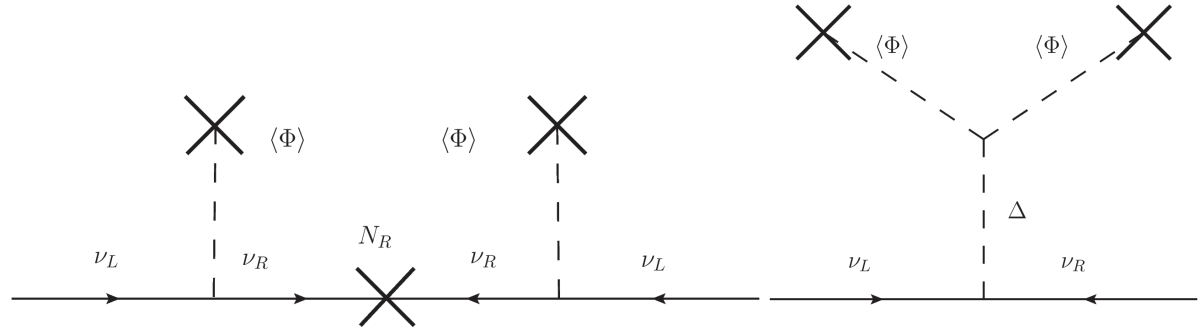
\includegraphics[height=3cm]{seesaw_feynman}
	\begin{minipage}[t]{0.6\textwidth}%{(a)}
		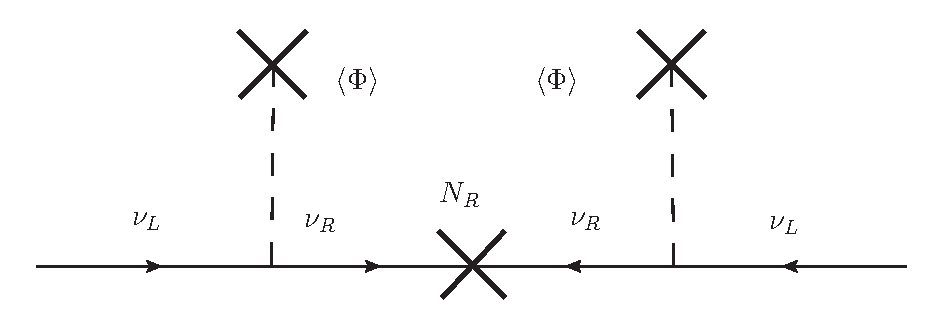
\includegraphics[width=8cm]{typeI_seesaw.eps}
	\end{minipage}
	\begin{minipage}[t]{0.3\textwidth}%{(b)}
		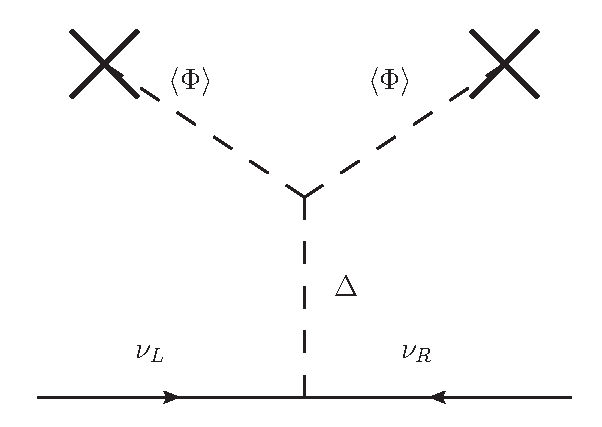
\includegraphics[height=3.0cm]{typeIIseesaw.eps}
	\end{minipage}
	\caption{ Tree-level Feynman diagrams for the Seesaw Mechanisms, modified from \cite{valle2015neutrinos}: type-I (left) and type-II (right). The type-III scheme shares the same diagram to the type-I, but with the $\nu_R$ replaced by $T^0$.}
	\label{seesaw}
\end{figure}

As a summary, to explain how the neutrinos acquire their masses, New Physics theories are required to extend the Standard Model. If neutrinos are Majorana particles, the induced Seesaw Mechanism can explain the tiny mass of the active neutrinos naturally. As a bonus, the mass scale required by the Seesaw Mechanism implies the New Physics in the GUT.



The results from the neutrino flavor transformation experiments proved that neutrinos are not massless and have finite masses. However, in these experiments, the mass differences, rather than the absolute mass values are measured so we can not know the absolute scale of neutrino masses from these results. Currently, there are mainly three approaches to probe the neutrino masses\cite{valle2015neutrinos}: (1) cosmological measurements\cite{dvorkin2019neutrino,gerbino2018status,aghanim2020planck}; (2) direct measurements of the $\beta$-decay spectrum; (3) a search for the $0\nu\beta\beta$ process. 

\subsection{Beta Decay}
In a $\beta$-decay process: $(Z,A)\to (Z+1,A)+e^-+\bar{\nu}_e$, parent nuclei with the nucleon number A and the proton number Z decay into daughter nuclei and electrons. By using the Fermi's Golden Rule, the differential $\beta^-$-decay spectrum of $T_e$ is given by\cite{rottele2019tritium}:
\begin{equation}\label{eq:beta-decay}
\begin{aligned}
\frac{d^2N}{dtdT_e} = \frac{G_F^2\cos^2\theta_C|\mathcal{M}_{nucl}|^2}{2\pi^3} &\cdot F(Z+1,T_e)\cdot(T_e+m_e)\cdot p_e\cdot (E_0-T_e)\\
&
\cdot \sqrt{(E_0-T_e)^2-m^2_{\bar{\nu}_e}}\Theta(E_0-T_e-m_{\bar{\nu}_e}),
\end{aligned}
\end{equation}
where $G_F$ is the Fermi constant; $\theta_C$ is the Cabibbo angle; $\mathcal{M}_{nucl}$ is the nuclear matrix element (NME); $F(Z,E)$ is the Fermi function describing the electromagnetic interaction between the $\beta$-electron and the final-state nucleus; and the Heaviside step function $\Theta$ ensures that a neutrino can only be emitted if enough energy is left for its mass.

The energy difference between the initial and final state nuclei is 

the sum of the emitted electrons $e^-$ (called the $\beta$-electron ) energy $E_e$, 

the antineutrino $\bar{\nu}_e$ energy $E_\nu$ and the nuclear recoil energy $E_R$: $Q=E_e+E_\nu+E_R$. If considering the initial and final nuclei are at rest and $E_R$ is negligible, due to the presence of $E_\nu$, $E_e$ can range from 0 to the maximal energy $E_0=Q$ (called the end-point energy). For the $\beta$-electron with a rest mass $m_e$, the kinetic energy $T_e=E_e-m_e$ (taking the natural unit $\hbar=c=1$) and the momentum $p_e=\sqrt{E^2+2Em_e}$. 


In this spectrum, $m^2_{\bar{\nu}_e}$, the square of the $\bar{\nu}_e$ rest mass is the measurement observable. It can be evaluated by measuring the $\beta$-decay event rate\cite{rottele2019tritium}.

If considering $m_{\nu_e}=m_{\bar{\nu}_e}$ and the CPT is conserved, $\langle m^2_{\bar{\nu}_e}\rangle=\langle m^2_{{\nu}_e}\rangle=\sum_i |U_{ei}|^2 m_i^2=\sum_i |U_{ei}|^2 m_i^2$. Taking out the lightest mass eigenvalue: $m_1$ for normal hierarchy and $m_3$ for inverted hierarchy, the $\langle m^2_{\nu_e}\rangle$ can be expressed as\cite{suekane2015neutrino}:
\begin{equation}\label{nuMassSquare}
\langle m^2_{\nu_e}\rangle = 
\begin{cases}
m_1^2+s^2_{13}|\Delta m^2_{31}|+c^2_{13}s^2_{12}\Delta m^2_{21}~(\mathrm{for~NH})\\
m_3^2+c^2_{13}|\Delta m^2_{31}|+c^2_{13}s^2_{12}\Delta m^2_{21}~(\mathrm{for~IH}),
\end{cases}
\end{equation}
where $s^2_{13}, c^2_{13}, \Delta m^2_{31}$ and $\Delta m^2_{21}$ are the flavor transformation parameters and they are determined by flavor transformation experiments. If taking the currently best global-fit values with $3\sigma$ (the values in brackets are for IH and the others are for NH): $\Delta m^2_{21}= 7.37 \times 10^{-5}~eV^2,~|\Delta m^2_{31}|= 2.56~(2.54)\times 10^{-3}~eV^2 ,s^2_{12}= 0.297, s^2_{13}= 0.0215~(0.0216)$\cite{pdg2020}, then  for NH, $\langle m^2_{\nu_e}\rangle \simeq m_1^2+(8.74~meV)^2$ and for IH, $\langle m^2_{\nu_e}\rangle \simeq m_3^2+(50.3~meV)^2$.
Fig.~\ref{lightestM} plots the $\sqrt{\langle m^2_{\nu_e}\rangle}$ as a function of the lightest mass eigenvalue.
\begin{figure}[htbp]\label{lightestM}
	\centering	
	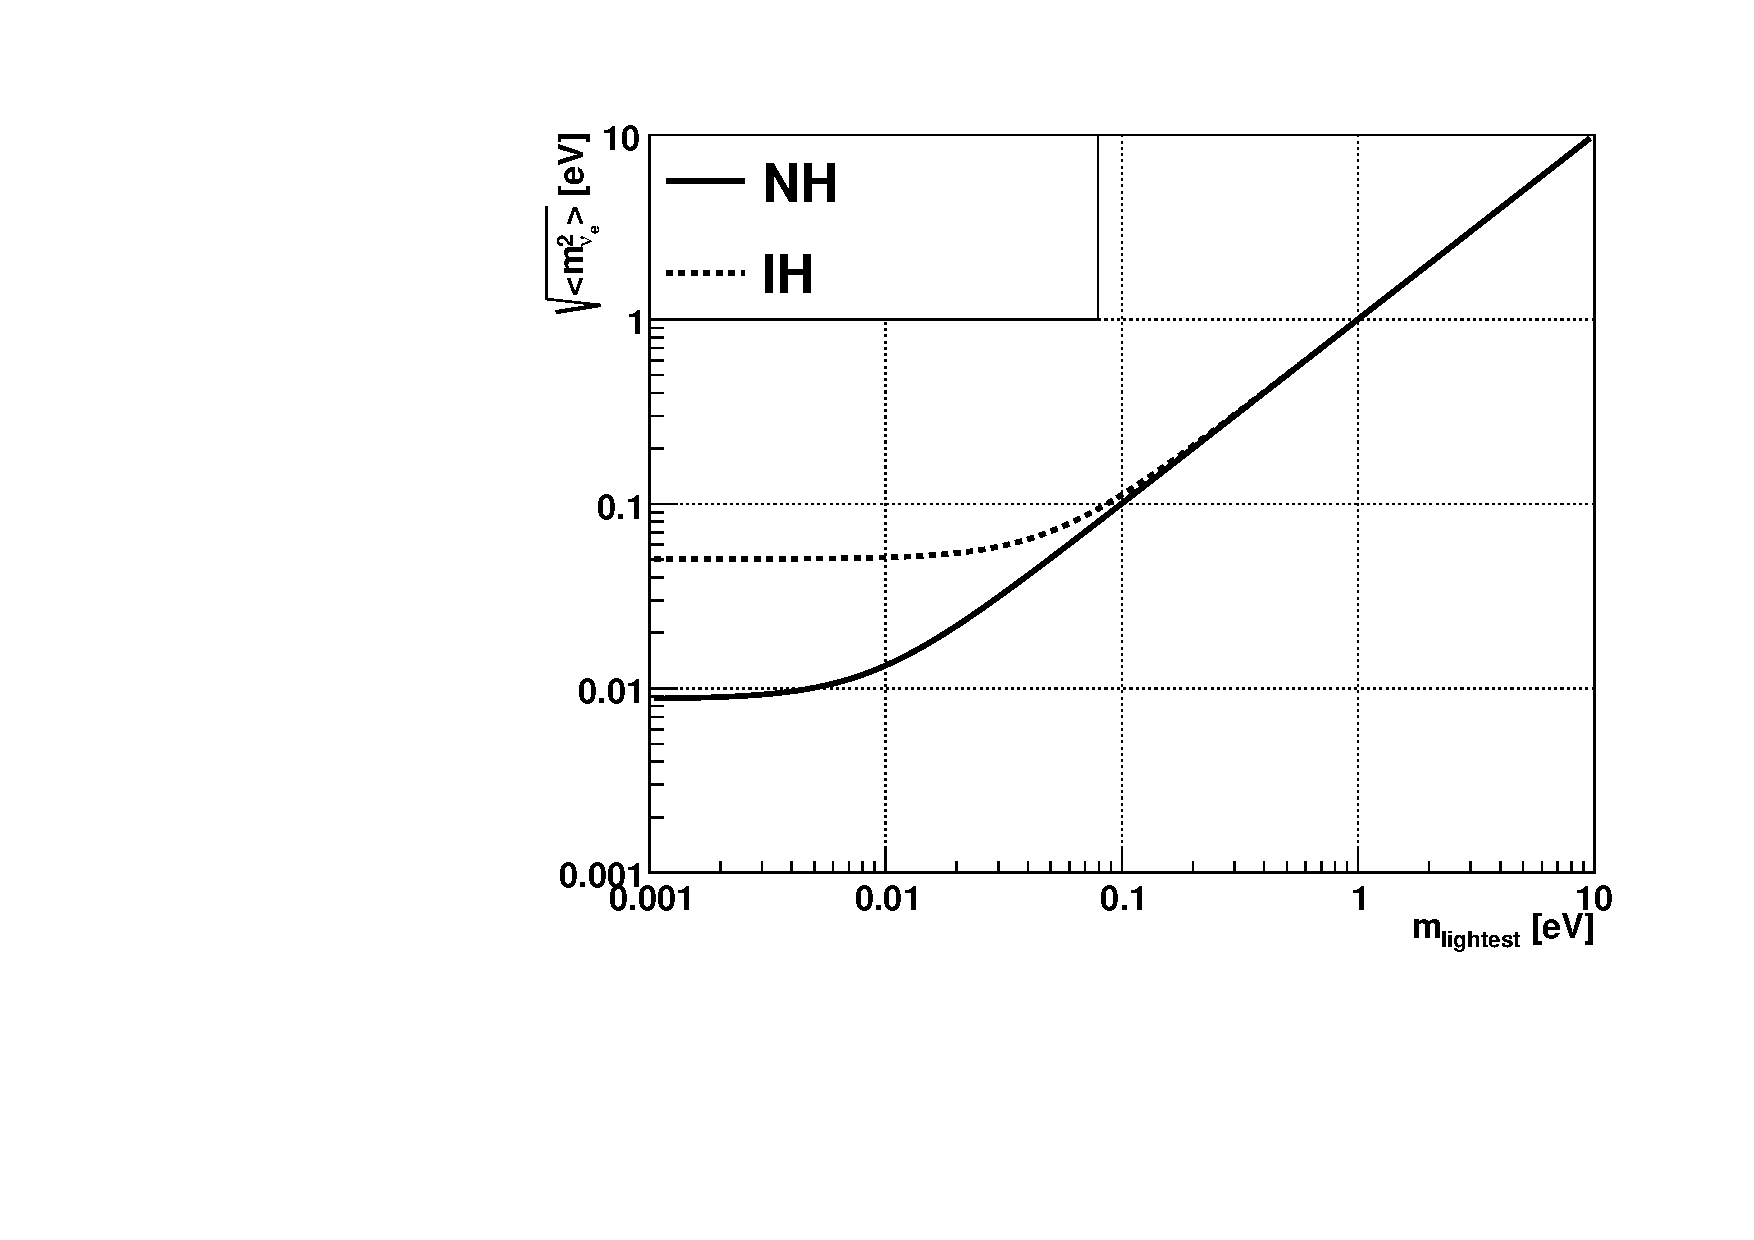
\includegraphics[width=10cm]{nu_massHierarchy.pdf}
	\caption{$\sqrt{\langle m^2_{\nu_e}\rangle}$ as a function of the lightest mass ($m_1$ for NH or $m_3$ for IH).}
	\label{nuMass}
\end{figure}
Therefore, once the $m^2_{\bar{\nu}_e}$ is measured, the mass hierarchy as well as the mass eigenvalues $m_i$ can be determined.

Among the $\beta$-decay processes, the tritium process: $^3$H$\to^3$He$^+$+$e^-+\bar{\nu}_e$ has a low endpoint energy $E_0=18.57$ keV, a favorable half-life $T_{1/2}=12.32$ years and simple atomic structure for calculation. With these experimental advantages, it has been largely investigated since 1947 and is used as a standard technology for the kinetic measurement\cite{fukugita2013physics}. The KArlsruhe TRItium Neutrino (KATRIN) experiment is one of the state-of-the-art tritium experiments which uses a large magnetic spectrometer with high energy resolution for precise measurement. In 2019, the experiment reported an upper limit of $m_\nu<1.1$ eV with 90\% C.L.. After 5 years of measurement, the experiment is expected to reach the $m_\nu$ sensitivity down to 0.2 eV with 90\% C.L.\cite{aker2019improved}.

\subsection{Double Beta Decay}
For heavy radioactive isotopes ($A>70$) with nuclei of even neutron number and even proton number (called the even-even nucleus), beta decay will lead to an odd-odd nucleus which is less stable. Thus for such isotopes, the $\beta$-decay is energetically forbidden. In 1935, Maria Goeppert-Mayer pointed out that these isotopes can still decay through a double beta decay process: $(Z,A) \to (Z+2,A)+2e^{-}+2\bar{\nu}_e+Q_{\beta\beta}$, where $Q_{\beta\beta}$ is the released energy. This is called ordinary double beta decay or $2\nu\beta\beta$, which is allowed by the Standard Model and with a typical half-life $T_{1/2}>10^{19}$ years (yr)\cite{povh2008particles,martin2019nuclear}.

If neutrinos are Majorana particles, a process called neutrinoless double beta decay ($0\nu\beta\beta$) will also be expected: $(Z,A) \to (Z+2,A)+2e^{-}+Q_{\beta\beta}$. In this process, the lepton number is violated by 2, which is not allowed in the SM. As mentioned in \ref{section:Majorana}, New Physics interpretations for the process are required. The Feynman diagrams of $2\nu\beta\beta$ and $0\nu\beta\beta$ are illustrated in Fig.~\ref{feynman1}.
\begin{figure}[htbp]
	\centering
	{	
	\begin{minipage}[t]{0.45\textwidth}{(a)}
		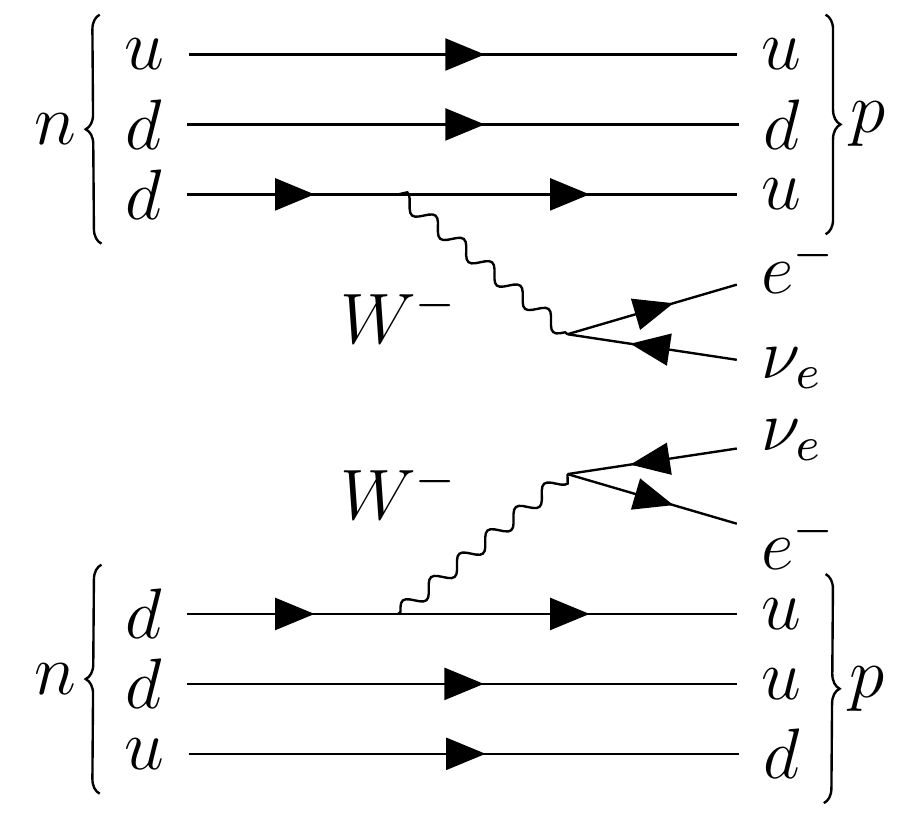
\includegraphics[width=5cm]{doubleBeta2nu_feynman.png}
	\end{minipage}
	\begin{minipage}[t]{0.45\textwidth}{(b)}
		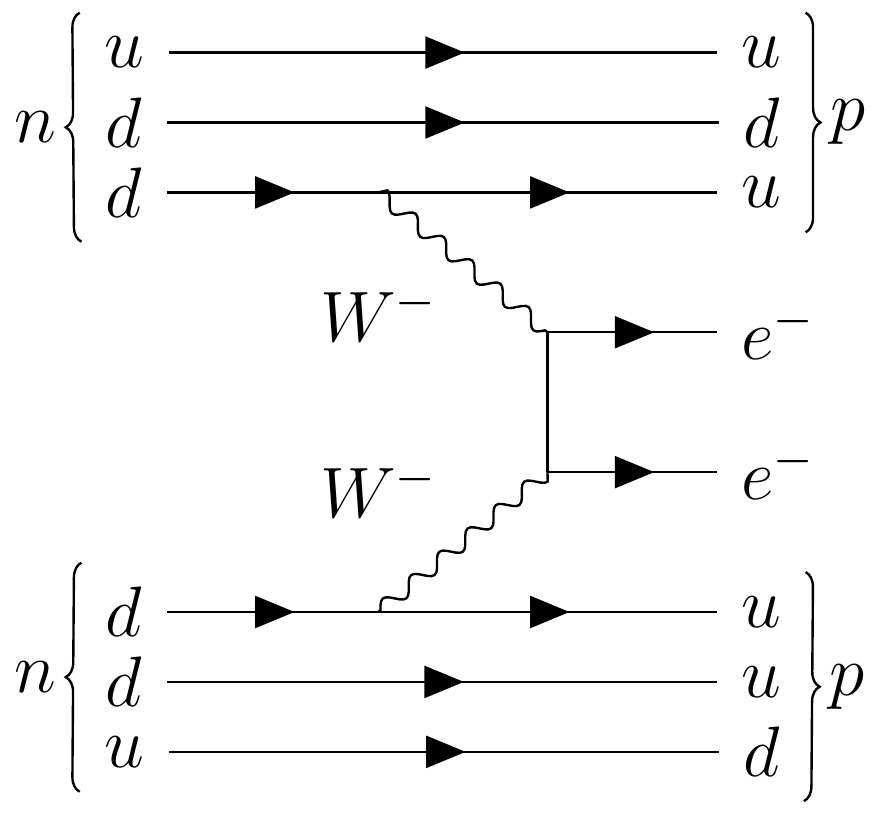
\includegraphics[width=5cm]{doubleBeta_feynman.png}
	\end{minipage}
	\caption{ Feynman diagrams for $2\nu\beta\beta$ (a) and $0\nu\beta\beta$ (b).}
	\label{feynman1}
}
\end{figure}

One of the simple interpretations is the exchanging of virtual light Majorana neutrinos between the nucleus, as shown in Fig.~\ref{feynman1} (b). Under the SM weak interactions, the amplitude of the lepton processes in the $0\nu\beta\beta$ is a product of two weak charged current interactions happening at the vertices $x$ (creating a $\nu_{eL}$ and an $e^-$) and $y$ (absorbing a $\nu_{eL}$ and creating an $e^-$) \cite{antonio2018state}:
\begin{equation}
\mathcal{A}=\bar{e}(x)\gamma^\mu\nu_{eL}\nu^T_{eL}(y)\gamma_\mu^T\bar{e}^T(y),
\end{equation}

Taking account of the three-neutrino mixing as well as the Majorana condition: $\nu_i^c=\mathcal{C}\bar{\nu}_i^T=\nu_i$,
 the amplitude becomes\cite{antonio2018state,bilenky2018introduction}:
\begin{equation}
\mathcal{A}=-\sum^3_{i=1}U^2_{ei}\frac{1-\gamma_5}{2}\nu_i(x)\bar{\nu}_i(y)  \frac{1-\gamma_5}{2}\mathcal{C}
\end{equation}

is propagator for a mass $m_i$ virtual fermion transiting between vertices. 

For the case of small neutrino mass, $p\gg m_i$, then $\mathcal{A}\propto m_{ee}\equiv \sum^3_{i=1}U^2_{ei}m_i$

the effective Majorana mass 

$\nu_i(x)\bar{\nu}_i(y)$ with a proper time ordering:

$\langle T(\nu_i(x)\bar{\nu}_i(y))=-\frac{i}{(2\pi)^4}\int dp^4 e^{-iq(x-y)}\frac{\gamma^\mu p_\mu+m_i}{p^2-m_i^2}$

$=-\sum^3_{i=1}U^2_{ei}m_i\frac{1}{p^2-m_i^2}\frac{1-\gamma_5}{2}\mathcal{C}.$

Therefore, the massive Majorana neutrino is required for the existence of the $0\nu\beta\beta$ process.
%where \cite{dolinski2019neutrinoless}.

From \cite{pdg2020}, transition between $\bar{\nu}_{eR}$ and $\nu_{eL}$.
%underlying mechanisms 

$|\bar{\nu}_{eR} (t=\delta t)\rangle  =|\bar{\nu}_{eR}\rangle-i\sum^3_{i=1}m_i U_{ei}|\nu_{iL} \rangle\delta t$

amplitude $\langle \nu_{eL}|\bar{\nu}_{eR}\rangle=-i\sum^3_{i=1}m_iU^2_{ei}\delta t$

Integrating the $\delta t$ with a weight of the nuclear matrix element, the decay width and the half-life are obtained as\cite{suekane2015neutrino,zuber2020neutrino}:
\begin{equation}
\Gamma=(T^{0\nu\beta\beta}_{1/2})^{-1} = G_{PS}(Q,Z)|M_{Nuclear}|^2\langle m_{ee}\rangle^2, 
\end{equation}
where $G_{PS}(Q,Z)$ is a phase space corresponding to the effective coupling constant, which depends on the endpoint energy $Q$ and the atomic number $Z$; $|M_{Nuclear}|$ is the nuclear matrix element describing the nuclear transition and it can only be calculated theoretically from approximate methods based on many-body nuclear models, such as the Nuclear Shell Model (NSM),


 interacting shell model (ISM)
 the Quasiparticle-Random Phase Approximation (QRPA), 

Interacting Boson Model (IBM), Energy Density Functional Method (EDF), and Projected Hartree-Fock-Bogoliubov Method (PHFB).

In this case the effective Majorana mass 
\begin{equation}
\langle m_{ee}\rangle = |\sum_{i=1}^3 U^2_{ei}m_i|= |c^2_{13}c^2_{12}m_1+c^2_{13}s^2_{12}e^{i\alpha_1}m_2+s^2_{13}e^{i\alpha_2}m_3|,
\end{equation}
where $U_{ei}$ are the elements of the neutrino mixing matrix for the flavor state $\nu_e$, and $m_i$ are the mass eigenvalues of the mass eigenstates (\ref{eq:mixingmatrix}));
$\alpha_1,\alpha_2$ are Majorana CP-violation phase factors and $\alpha_2$ can also be taken as $\alpha_2-\delta_{CP}$.

For NH, $m_{lightest}=m_1$,
$m_2=\sqrt{m_1^2+\Delta m^2_{21}}, m_3 = \sqrt{m_1^2+|\Delta m^2_{31}|}$;
for IH, $m_{lightest}=m_3$,
$m_1=\sqrt{m_3^2+|\Delta m^2_{31}|}, m_2=\sqrt{m_3^2+|\Delta m^2_{31}|+\Delta m^2_{21}}$

The phases $\alpha$ and $\beta$ are ranging from 0 to $\pi$, taking different pairs of $(\alpha_1,\alpha_2)=(0,0),(0,\pi), (\pi, 0)$ and $(\pi,\pi)$ can determine the ranges of $\langle m_{ee} \rangle$.


Using the same best-fit values in the \ref{section:directMeasure}, a plot of $\langle m_{ee}\rangle$
as a function of $m_{lightest}$ is shown in Fig.~\ref{effectiveMajorana}. 


the mass regions are bounded by lines taking different values of $(\alpha_1,\alpha_2)$.

\begin{figure}[htbp]\label{effectiveMajorana}
	\centering	
	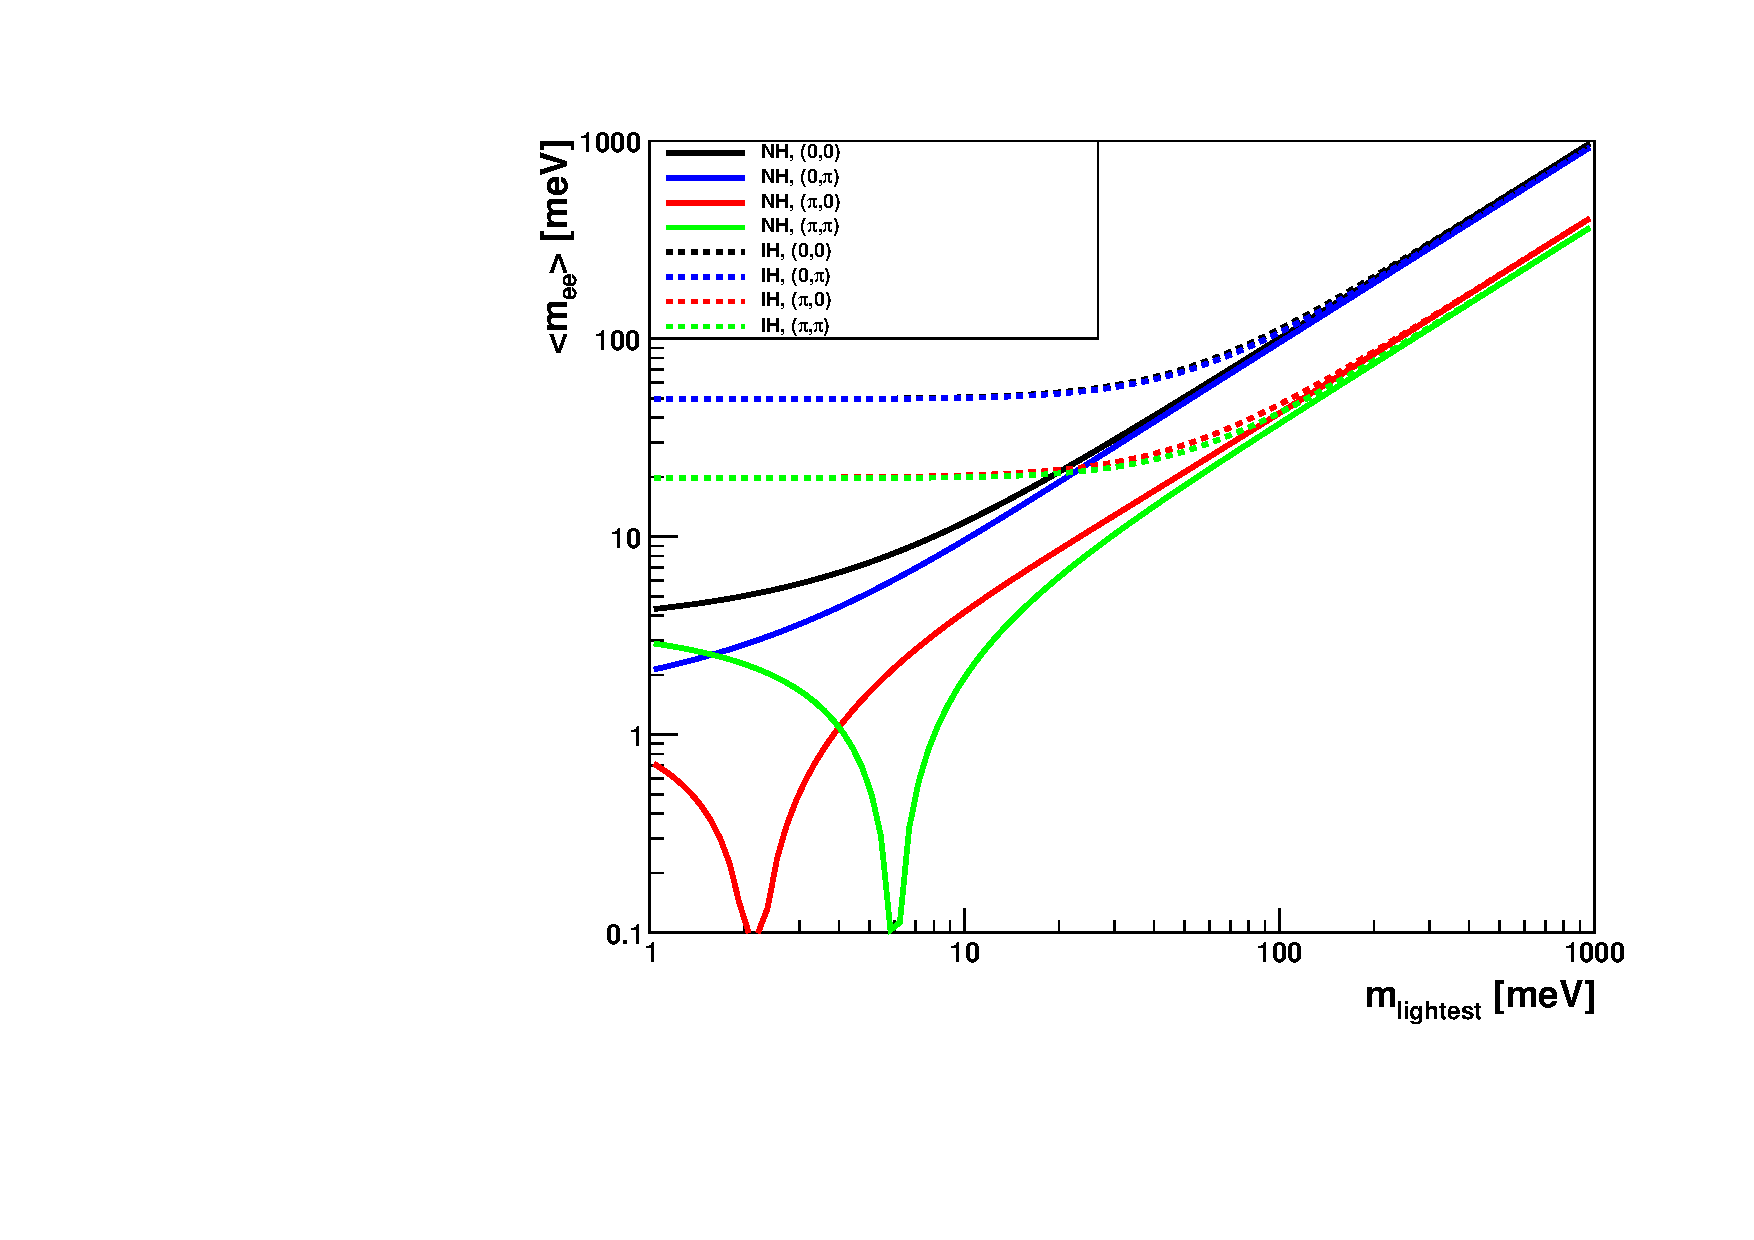
\includegraphics[width=12cm]{effectiveMassPlots.pdf}
	\caption{Effective Majorana mass as a function of the lightest mass eigenvalue. Solid lines are for NH cases and dashed lines are for IH. Different colors stand for taking different values of $(\alpha_1,\alpha_2)$.}
	\label{effectiveMass}
\end{figure}

Similar to the $\beta$-decay case, the $2\nu\beta\beta$ process will cause a continuous spectrum in the detector while the $0\nu\beta\beta$ process only has two electrons in the final state. These electrons take away the entire energy and their energy spectrum sum up to give a distinct energy peak at the Q-value. 
Taking the isotope $^{130}$Te as an example, Fig.~\ref{te130energy} illustrates the shapes of the energy spectrum from the $2\nu\beta\beta$ and the $0\nu\beta\beta$ decay processes.

By measuring this distinct energy peak, a detector with high energy resolution can search for the $0\nu\beta\beta$ signal from the $0\nu\beta\beta$ decay radioactive isotopes. Diverse technologies have been developed during the past decades. The following section lists some of the mainstream experiments.

\begin{figure}[htbp]
	\centering	
	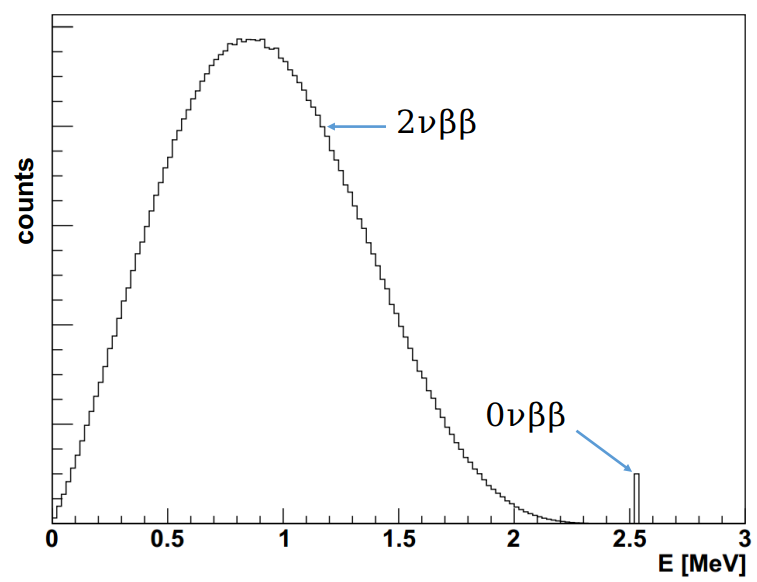
\includegraphics[width=8cm]{Te130_energy0vbb.png}
	\caption{Energy spectrum of the $^{130}$Te $2\nu\beta\beta$ decay and the hypothetical $0\nu\beta\beta$ decay. The SNO+ simulation package (RAT) was used to produce the plot.}
	\label{te130energy}
\end{figure}

The signal of $0\nu\beta\beta$ in the range of $10^{25}-10^{26}$ year,

The observed number of event in expectation is: 
\[
N_{event} = \ln 2 \frac{N_A}{M_A}\frac{\alpha\cdot\epsilon\cdot m\cdot t}{T^{0\nu}_{1/2}},
\]

where $N_A$ is the Avogadro's number, $\alpha$ is the abundance of the isotope in the element, 
$M$ is the molar mass of the isotope and $t$ is the measurement time of total exposure.



\subsubsection{Status of Double Beta Decay Experiments}

There are 35 isotopes can undergo the double beta decay process, but only a few of them are suitable for the application in direct $0\nu\beta\beta$ search experiments\cite{giunti2007fundamentals}. From the experimental view, the candidate isotopes are expected to have relatively high natural abundances, high Q-values, be deployed in a large amount with low costs, not toxic to the environment, and etc. However, in a realistic situation, no isotope fulfills all these properties, and trade-offs have to be made for the current experiments\cite{dolinski2019neutrinoless}. The experiments discussed below are using the $^{76}$Ge, $^{136}$Xe and $^{130}$Te isotopes.

\begin{figure}[!htb]
	\centering
	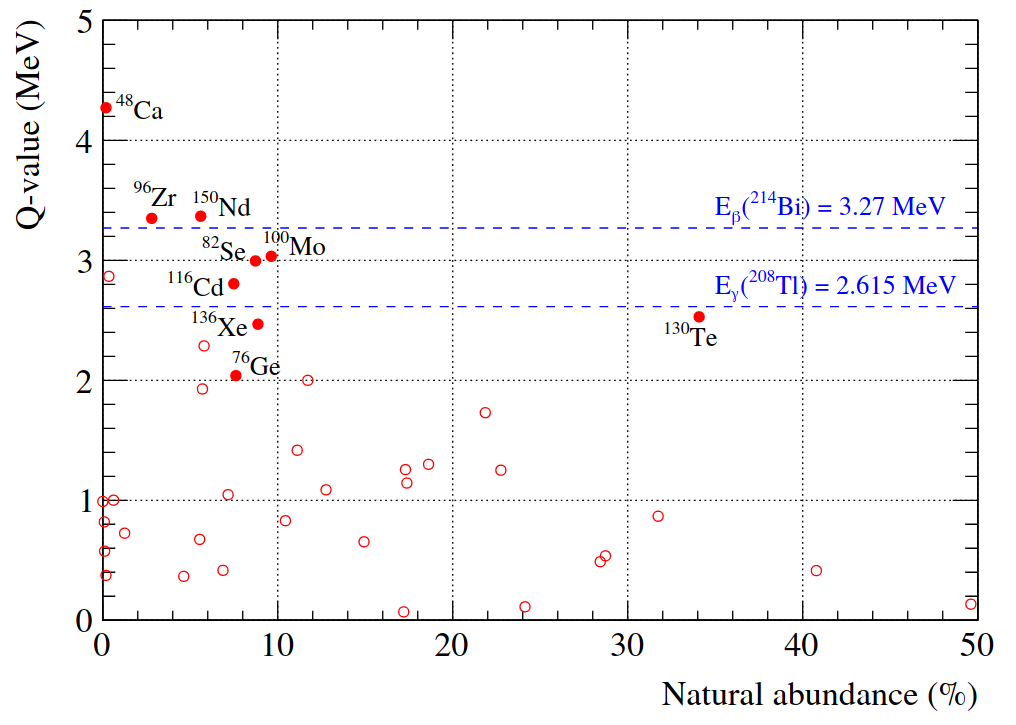
\includegraphics[width=10cm]{Te_abundance.png}
	\caption{Natural abundance vs. Q-values for different $2\nu\beta\beta$ isotopes\cite{snop_nim}.}
	\label{te_abundance}
\end{figure}

searching for direct signals of $0\nu\beta\beta$ mainly measure the physics properties of the two emitted electrons, such as their energies, momentum, and tracks. 

\begin{itemize}
	\item  $^{76}$Ge

The GERmanium Detector Array (GERDA) experiment is located at Gran Sasso National Laboratories (LNGS). It uses bare germanium crystals with enrichment of up to $\sim$87\% $^{76}$Ge operated in a radiopure cryogenic liquid argon (LAr)\cite{agostini2016search}. GERDA Phase I had an exposure of 21.6 kg$\cdot$yr and Phase-II started with 35.6kg from enriched material in December 2015. With combined data of Phase I and Phase II, a total exposure of 82.4 kg$\cdot$yr has been measured.

In 2019, GERDA reported a lower limit half-life of $T^{0\nu}_{1/2}(^{76}$Ge$)>0.9\times 10^{26}$ years at 90\% C.L. with an effective $m_{ee}$ in [104,228]~meV\cite{agostini2019probing}.

Based on the experiences from the GERDA and the MAJORANA DEMONSTRATOR experiment, a new experiment, the Large Enriched Germanium Experiment for Neutrinoless Double-Beta Decay (LEGEND) will pursue a tonne-scale by using the Inverted-Coaxial Point Contact (ICPC) detector. It has discovery potentials at a $T_{1/2}^{0\nu\beta\beta}>10^{28}$ years\cite{elliott2019legend}.

\item $^{136}$Xe
	
The Enriched Xenon Observatory (EXO) experiment uses 200-kg liquid Xenon (LXe) time projection chamber (TPC) to search for $0\nu\beta\beta$ in $^{136}$Xe. In 2011 they observed the half life of double beta decay of $^{136}$Xe to be $2.11\times 10^{21}$ years and in 2014 they set a limit on $T^{0\nu}_{1/2}(^{136}$Xe$)>1.1\times 10^{25}$ yr\cite{albert2014search}. EXO is now upgrading to the next 5-tonne experiment (nEXO) and is expected to reach an exclusion sensitivity of $T^{0\nu}_{1/2}(^{136}$Xe) to about $10^{28}$ years at 90\% C.L.\cite{albert2018sensitivity}.

The Particle and Astrophysical Xenon Experiment located at China Jinping Underground
Laboratory also uses a high-pressure gas-phase time projection chamber (TPC) with Microbulk Micromegas, a fine pitch
micro-pattern gas detector as charge readout to reconstruct $0\nu\beta\beta$ event tracks.

. contain 200 kg, 90\% 136Xe enriched gas operated at 10 bar.
ultimate sensitivity after 3 years would reach $10^{27}$ years.
 $m_{0\nu\beta\beta}$ 20 to 50 meV 
\cite{han2020pandax}.

The KamLAND-Zen (ZEroNeutrino) experiment exploits the existing facilities of KamLAND by setting a 3.08-m-diameter spherical inner balloon filled with 13 tons of Xe-loaded liquid scintillator at the center of the KamLAND detector. The liquid scintillator is a cocktail of 82\% decane and 18\% pseudocumene by volume, 2.7 g/L PPO with a photocathode coverage of 34\%. Their 2016 results from a 504 kg$\cdot$yr exposure obtained a lower limit for the $0\nu\beta\beta$ decay half-life of $T^{0\nu}_{1/2}(^{136}$Xe$)>1.07\times 10^{26}$ yr at 90\% C.L. and the corresponding upper limits on the effective Majorana neutrino mass are in the range $61-165$ meV\cite{gando2016search}.

\item $^{130}$Te

The Cryogenic Underground Observatory for Rare Events (CUORE) experiment searches for $0\nu\beta\beta$ in $^{130}$Te. CUORE is a ton-scale cryogenic bolometer array that arranges 988 tellurium dioxide (TeO$_2$) crystals. CUORE reported its first results in 2017 after a total TeO$_2$ exposure of 86.3 kg$\cdot$yr. An effective energy resolution of ($7.7\pm 0.5$) keV FWHM and a background count of ($0.014\pm0.002$) $counts/(keV\cdot kg\cdot yr)$ in the ROI were achieved in that data exposure. Combined with the early data (the data from the two precursor experiments, Cuoricino and CUORE-0), they placed a lower limit of $T^{0\nu}_{1/2}(^{130}$Te$)>1.5\times 10^{25}$ yr at 90\% C.L. and $m_{\beta\beta}<(110-520)$ meV\cite{alduino2018first}. In 5 years live time, the experiment will give a projected sensitivity of $9.5\times 10^{25}$ yr at the 90\% C.L. and set an upper limit on the effective Majorana mass in the range $50-130$ meV\cite{piperno2015dark}.

Instead of using Te crystal and cryogenic technology, the SNO+ experiment uses a novel technology by dissolving the Te isotope into liquid scintillator. Details will be discussed in Chapter.~3.

\end{itemize}

A more recent evaluations of the limits of $T^{0\nu}_{1/2}$ and $m_{\beta\beta}$ from the above mentioned current and future experiments are summarized in Table.~\ref{gerdatable}\cite{agostini2017discovery,agostini2019probing}. The values below the double-line are 3$\sigma$ $0\nu\beta\beta$ discovery sensitivities assuming 5 years of live time for planned future experiments.%SNO+ Phase-I and II 
\begin{table}[ht]
	\centering
	\caption{\label{gerdatable} The limits of $T^{0\nu}_{1/2}$ and $m_{\beta\beta}$ at 90\% C.L.}	
	{
		\begin{tabular*}{135mm}{c@{\extracolsep{\fill}}cccc}
			\toprule 
			Experiment & Isotope & Limit of $T^{0\nu}_{1/2}$ ($10^{25}$ year) & Limit of $m_{\beta\beta}$ (eV)\\
			\midrule
			GERDA       & $^{76}$Ge & $>$8.0 & $<$0.12-0.26  \\	
			KamLAND-Zen & $^{136}$Xe & $>$10.7 & $<$0.05-0.16	\\
			EXO         & $^{136}$Xe & $>$1.1 & $<$0.17-0.49  \\	
			CUORE       & $^{130}$Te & $>$1.5 &  $<$0.11-0.50 \\
		   \hline		  
		   \hline
		    LEGEND-1k & $^{76}$Ge & 8.4 & 0.04-0.073\\
			KamLAND2-Zen & $^{136}$Xe &8.0 & 10.7 & 0.05-0.16	\\
			nEXO         & $^{136}$Xe &41.0 & 410 & 0.09-0.022  \\
			NEXT 1.5k& $^{136}$Xe& 1367 &  7.9 & 21-49\\
			PandaX-III 1k& $^{136}$Xe & 901& 9.0 & 20-46\\	
			CUPID       & $^{130}$Te& 543 & 21.0 &  11-26 \\
			SNO+ Phase I &$^{130}$Te& 1367  &1.1 & 46-115\\
			SNO+ Phase II &$^{130}$Te& 7960 &4.8 & 22-54\\
			\bottomrule	
		\end{tabular*}
	}
\end{table}
\vspace{1cm}

%\begin{table}[ht]
%	\caption{\label{newLimits} The limits of $T^{0\nu}_{1/2}$ and $m_{\beta\beta}$ at 90\% C.L.}	
%	{\centering
%		\begin{tabular*}{135mm}{c@{\extracolsep{\fill}}ccccc}
%			\toprule 
%			Experiment & Isotope & $m_{isotope}$ [kg] & $T^{0\nu}_{1/2}$ [$\times 10^{26}$ year] & $m_{\beta\beta}$ [meV]\\
%			\midrule
%
%			\bottomrule	
%		\end{tabular*}
%	}
%\end{table}
%\vspace{1cm}